\begin{frame}
\frametitle{Struttura di un messaggio ICMP} 
In un \textbf{Covert Channel ICMP} verranno utilizzati i messaggi ICMP per l'esfiltrazione dei dati.  Essi contengono un l'intestazione IP di base. Quindi i primi venti byte indicano l'intestazione IP mentre l'ultimo ottetto di byte riguarda l'intestazione ICMP.   
\end{frame}  
\begin{frame}{}
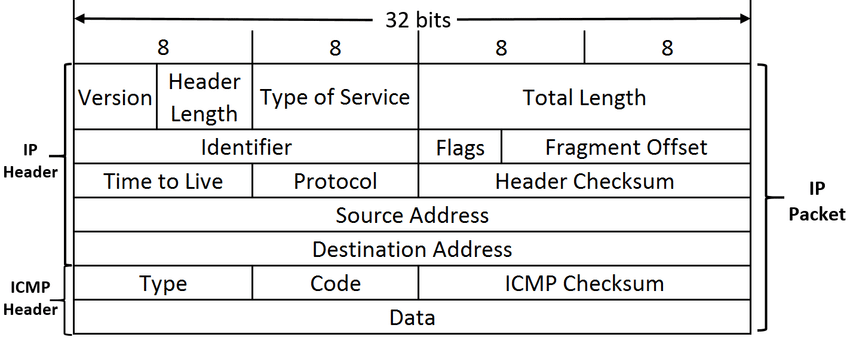
\includegraphics[width=0.8\textwidth]{../Tesi/img/ICMP-packet-structure.png} 
%\begin{itemize} 
 %\item \textbf{Type}: Identifica la tipologia di messaggio.  
%In base a questo campo verrà determinato il formato dei rimanenti dati. 
%\item \textbf{Code}: Fornisce dettagli aggiuntivi sulla tipologia di messaggio.
%\item \textbf{Checksum}: 
%Complemento a 16 bit relativo alla somma del messaggio ICMP. 
%Garantisce l'integrità dei dati. 
%\item \textbf{Data}: Campo opzionale, può contenere ulteriori dati. 
%Può contenere la parte del pacchetto IP originale che ha causato il messaggio o altre tipologie di dati. 
%\end{itemize} 
\end{frame} 
%\import{frames}{introduzione_ICMP_tipologie} 
